\subsection{Construction of semi physical demonstration}

We found a space at accenture that was big enough to build the track. Because of the limitations of the raspberry pi were the power given to the vehicles could not be under 40 and over 100 (We are not sure what the metrics is for power), we needed a road that could be over three meters long. If the road was under three meters the vehicle that had be given a power by the server which were under the limit. The server works in a way that the demo would not start until both vehicles had connected to it. Theoretically this means that the vehicles should start at the same time. We also placed the vehicles at the same lenght apart from the intersection so that they would crash if the server did not intervene. This way we could know for sure that the server were giving directions to the vehicles. 

To make the demo hundred percent accurate were not possible. This is beacause of the limitations of the raspberry pi. As mentioned it was not a vast gap between the lowest and the highest velocity of the vehicles. The vehicles were not able to recieve the messages at the excact same time as well. This ment that they could start with a difference of half a secound. Another factor was that the vehicles were not always moving completely straight forward which we assumed in the server. However we were able to get a consistent demo with enough margins. We made  vast margins by making a buffersone around the vehicles. The buffersone was about twenty centimeters. An example of a non-successful demo can be seen in figure 3.6.

\begin{figure}[h!]
	\centering
	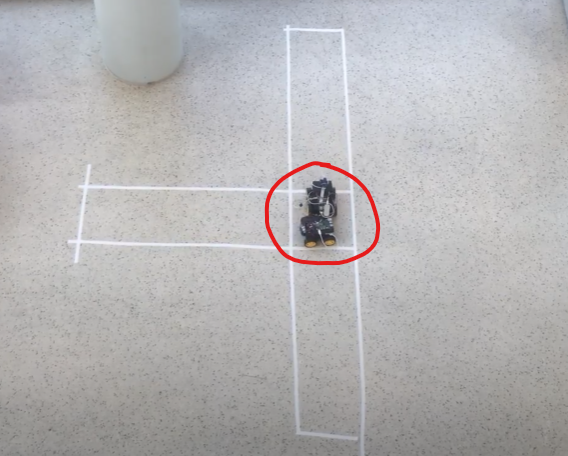
\includegraphics[width=1\linewidth]{figures/demo_crash}
	\caption[Crash in demo]{Here we can observe the two cars colliding in the intersection. The colliding happened because one of the cars started about 5 centimeters further behind than the other car as well as starting a few millisecounds after. Meanwhile the server assumed they startet at the excact same time at equal distance to the intersection. Those small errors led to a crash because we did not have enough margin for error in our demo yet.}
	\label{fig:crashdemo}
\end{figure}

After we implemented the buffersone we were able to get a consistent semi physical demonstration. Here is how a succesfull demo would go. When both cars connected to the server, they startet at the same velocity which were specificly set to 80cm/h in our demo. We decided on this velocity because it was the highest velocity that the Raspberry Pi cars could have, according to our previous measurments. Not long after they started, the server recognizes that the cars are near the intersection. Then the server calculates which car has to slow down and how much the car needs to slow down to avoid collision. The server calculates using the cars velocity, position and length. In our case the server calculated the velocity 55 cm/s which was the lowest possible velocity according to our measurements. Further the server sends its calculated velocity to the car that needs to slow down. The car that needs to slow down is the car that would enter last into the intersection. After the other car has supposedly passed the intersection the car that slowed down gets told by the server to speed up to its original velocity. An example of a successful demo can be seen in figure 3.7.


\begin{figure}[h!]
	\centering
	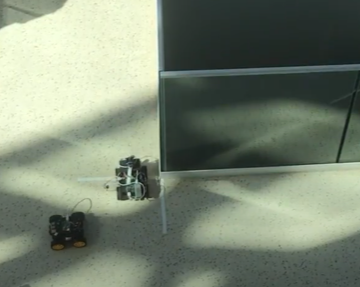
\includegraphics[width=1\linewidth]{figures/succsess_demo}
	\caption[Successful demo]{Here is a snipped from a successful demo. The car to the left has just passed the intersection which is marked by the white tape. The car furthest up is therfore about to accelerate up to its original velocity. Here we can observe that the margins where big enough to prevent the cars colliding}
	\label{fig:successdemo}
\end{figure}
